\subsection{RANSAC-Based Motion Filtering}
A key stage in the pipeline is filtering static landmarks from dynamic objects to ensure ego-motion estimation is based only on stable references.  
To achieve this, a RANSAC-based model is fitted to the relationship between azimuth angle $\theta$ and Doppler velocity $v_d$.

\paragraph{Principle and Theory}
Static reflections observed by a moving radar follow a predictable Doppler pattern:
\[
v_d = v_e \cos(\theta),
\]
where $v_e$ is the vehicle’s forward velocity and $\theta$ the azimuth angle relative to the vehicle heading.  
Objects directly ahead or behind ($\theta = 0^\circ, 180^\circ$) show the maximum Doppler shift ($v_d \approx \pm v_e$), while objects at $90^\circ$ yield $v_d \approx 0$.  
This results in a cosine-shaped distribution of radial velocities across azimuth.  

Dynamic targets deviate from this ideal distribution, whereas static reflections align closely with the curve.
In practice, the noisy radar points can be fit to this theoretical shape using estimation methods such as Least Mean Squares (LMS), which makes deviations more apparent.  

Figure~\ref{fig:self_speed_doppler} illustrates this concept with simulated data.  
The noisy radar points (red crosses) follow the expected cosine profile, while the LMS-estimated curve (purple dashed line) recovers the underlying shape and closely matches the ideal Doppler profile (blue line).  

\begin{figure}[!htbp]
    \centering
    \begin{subfigure}{0.48\linewidth}
        \centering
        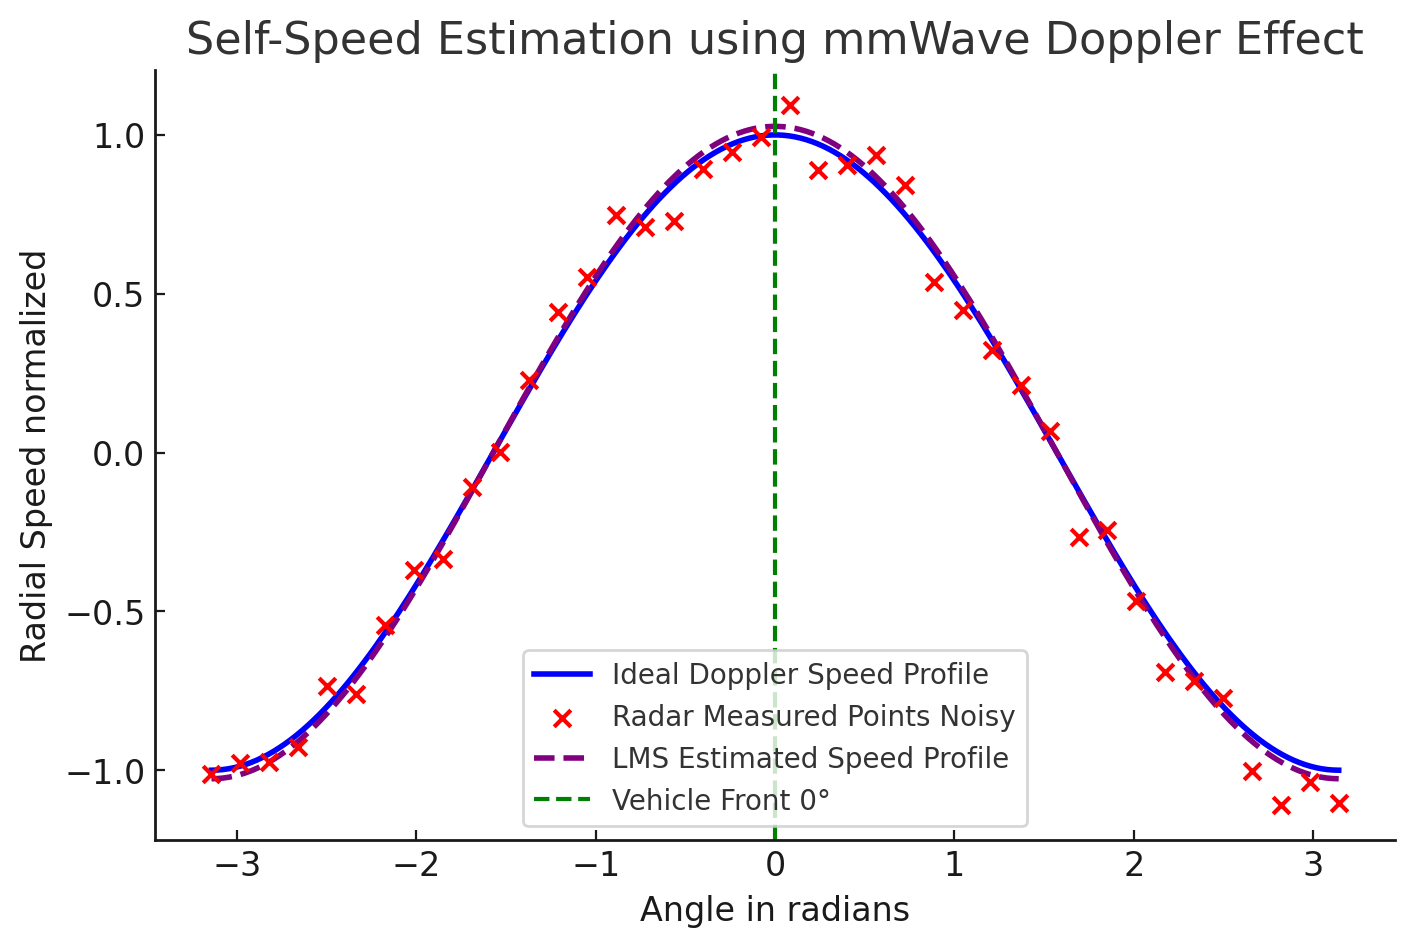
\includegraphics[width=\linewidth]{images/Self_Speed_Doppler.png}
        \caption{Simulated Doppler speed profile.  
        Red = noisy radar points, blue = ideal cosine distribution, green dashed = vehicle front ($\theta=90^\circ$).}
        \label{fig:self_speed_doppler}
    \end{subfigure}
    \hfill
    \begin{subfigure}{0.48\linewidth}
        \centering
        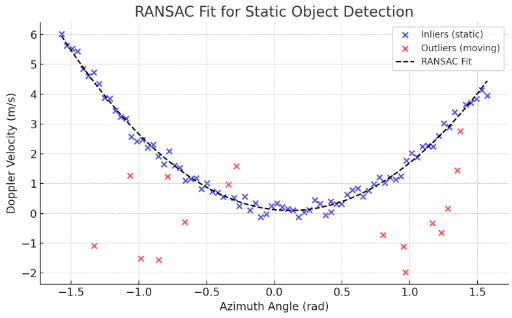
\includegraphics[width=\linewidth]{images/RANSAC.png}
        \caption{Simulated RANSAC fit of Doppler vs.\ azimuth.  
        Blue = static inliers, red = moving outliers.}
        \label{fig:ransac_simulated}
    \end{subfigure}
    \caption{Simulated validation of Doppler-based self-speed estimation.  
    (a) shows the expected cosine-shaped Doppler profile of static objects with LMS fitting,  
    while (b) demonstrates RANSAC filtering to separate static inliers from dynamic outliers.}
    \label{fig:simulated_doppler_ransac}
\end{figure}


\paragraph{Implementation}
In practice, the radar provides pairs $(\theta, v_d)$ of azimuth and Doppler velocity for each detected point.  
The ego-velocity $v_e$ is unknown and must be estimated from these observations.  
The theoretical relationship is
\[
v_d = v_e \cos(\theta),
\]
where static reflections align along a cosine-shaped Doppler profile.  
However, directly fitting a cosine to noisy radar data with outliers is unstable and highly sensitive to dynamic targets.  

To address this, the Doppler profile is instead approximated by a quadratic function:
\[
v_d = a\theta^2 + b\theta + c,
\]
fitted robustly with a \textbf{RANSACRegressor}.  
This approximation leverages the fact that within the radar field of view, the cosine curve can be closely represented by a parabola as shown in Figure~\ref{fig:ransac_simulated}, while RANSAC rejects inconsistent points caused by moving objects.  

The algorithm iteratively:
\begin{enumerate}
    \item Samples small subsets of $(\theta, v_d)$ pairs.
    \item Fits a quadratic model.
    \item Evaluates inliers based on residual error.
    \item Selects the model with maximum consensus.
\end{enumerate}

Once the model is fitted, the \textbf{ego-velocity $v_e$} is extracted from the amplitude of the fitted curve at $\theta = 0$, corresponding to the radar’s forward direction.  
Inliers are classified as static reflections and provide a reliable basis for ego-motion estimation, while outliers correspond to dynamic objects that are excluded from the calculation.

\begin{figure}[!htbp]
    \centering
    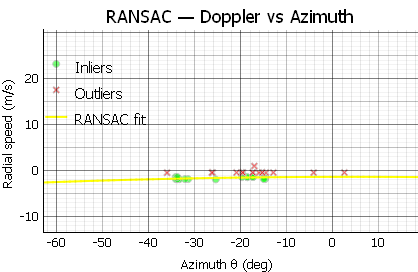
\includegraphics[width=0.9\linewidth]{images/RANSAC_movingTarget_wPtCloud.png}
    \caption{Real implementation of RANSAC filtering: green = static inliers, red = dynamic outliers.}
    \label{fig:ransac_real_static_dynamic}
\end{figure}

\newpage
\paragraph{Pipeline Role}
As illustrated in the system pipeline (Fig.~\ref{fig:dual_radar_pipeline}), the RANSAC filter is positioned after static thresholding and before ego-velocity estimation.  
Its primary purpose at this stage is to separate dynamic objects from static landmarks, ensuring that subsequent modules operate only on consistent and reliable data.  

Without this step, moving objects would propagate through clustering and ICP, corrupting the estimation of ego-motion.  
By filtering out dynamic outliers, RANSAC guarantees that only stable reflections are retained for trajectory alignment and speed estimation.  
\vspace{0.5em}
The output of this stage is therefore two-fold:
\begin{itemize}
    \item A refined set of static landmarks, which serve as input for clustering and ICP-based odometry,
    \item A clean separation of dynamic actors, preventing them from biasing ego-motion estimation.
\end{itemize}
